\documentclass{ieeeaccess}

\usepackage{cite}
\usepackage{amsmath,amssymb,amsfonts}
\usepackage{algorithmic}
\usepackage{graphicx}
\usepackage{textcomp}
\usepackage{booktabs}
\usepackage{multirow}
\usepackage{array}
\usepackage{xcolor}
\usepackage{url}
\usepackage{bm}
\usepackage{microtype}

\graphicspath{{figures/}}
\setlength{\emergencystretch}{2em}
\makeatletter
\setlength{\@dblfptop}{0pt}
\setlength{\@dblfpsep}{14pt}
\setlength{\@dblfpbot}{0pt plus 1fil}
\makeatother

\newcommand{\dasp}{DASP}
\newcommand{\ssf}{SSF-budget}
\newcommand{\earlyf}{EarlyMacroF1@5}
\newcommand{\earlyr}{EarlyAttackRecall@5}
\newcommand{\discussionhead}[1]{%
  \par\addvspace{7pt}%
  \noindent{\color{greycolor}\bfseries\itshape #1}\par\nobreak\vspace{1pt}\nobreak}

\def\BibTeX{{\rm B\kern-.05em{\sc i\kern-.025em b}\kern-.08em
T\kern-.1667em\lower.7ex\hbox{E}\kern-.125emX}}

\begin{document}

\vol{XX}
\year{2026}
\history{Submission metadata to be completed by the authors.}
\doi{To be assigned after acceptance}

\title{DASP: Drift-Triggered Selective Layer Adaptation for Streaming Network Intrusion Detection}

\author{\uppercase{Author Name}\authorrefmark{1}}
\address[1]{Affiliation to be completed before submission (e-mail: corresponding author e-mail to be completed).}
\tfootnote{The author list, affiliations, funding statement, and acknowledgments must be verified before submission.}
\markboth{Author Name: DASP for Drift-Adaptive Network Intrusion Detection}{Author Name: DASP for Drift-Adaptive Network Intrusion Detection}
\corresp{Corresponding author: Author Name (e-mail: to be completed).}

\begin{abstract}
Evaluation of drift-adaptive network intrusion detection is vulnerable to temporal leakage, unequal label budgets, and statistical analyses that treat stream windows as independent replicates. This study presents DASP, a prediction-first streaming detector that freezes its base multilayer perceptron after warm-up and adapts low-rank layer branches, feature-wise residual modulators, an input adapter, and the classifier through event-gated fast and strong paths. DASP combines multilevel feature monitoring, delayed-performance triggering, current-batch similarity replay, label-blind uncertainty and novelty queries, class-balanced candidate guards, and a fused inference cache. The controlled confirmation contains 400 runs on NF-UNSW-NB15-v3: five class-conditional composition-shift scenarios, five stream seeds, two model seeds, DASP, and seven locked comparators. Labels are delayed by one window and each method receives at most 256 ground-truth update labels per window. DASP obtained the highest mean early post-shift macro-F1 (0.995543). Its prespecified effect over SSF-budget was 0.001726 (95\% hierarchical-bootstrap CI $[0.001522,\,0.002039]$), but an exact two-sided sign-flip test over the five independent stream clusters gave $p=0.0625$. No exploratory DASP--baseline comparison survived Holm correction. A frozen A-trained probe showed no binary-boundary degradation on the NF-UNSW shift artifacts, so these data establish distribution-shift stress testing rather than real-concept-drift adaptation. Detector precision and recall were only 0.1667 and 0.1800. A separate 80-run GPU benchmark showed that DASP had the fastest p95 forward inference (3.675 ms per 4,096-flow window), but ranked fifth in complete test-then-train latency (47.558 ms mean; 87,041 flows/s) because selective adaptation produced a long update tail. No DASP run performed a base-backbone or global update. The evidence supports an accuracy--efficiency trade-off and auditable selective adaptation, but not causal trigger benefit, cross-dataset generality, or superiority.
\end{abstract}

\begin{keywords}
Concept drift, continual learning, delayed labels, intrusion detection, low-rank adapters, network flows, prequential evaluation, selective layer adaptation.
\end{keywords}

\titlepgskip=-15pt
\maketitle

\section{Introduction}
\label{sec:introduction}

\PARstart{N}{etwork} intrusion detectors operate in environments whose services, traffic volumes, and attack behaviors change over time. A model trained once can therefore lose predictive validity even when its original held-out score was high. Concept drift is commonly expressed as a temporal change in $P_t(X,Y)$ through the feature distribution, the conditional label relationship, or both \cite{Gama2014ConceptDrift}. Abrupt, gradual, recurring, and local changes impose different adaptation requirements \cite{Li2024DriftType,Aguiar2024Locality}.

Experimental design determines whether adaptation is actually measured. Random train--test splits remove the temporal dependence that defines drift. Training on a window before scoring it exposes current labels to the prediction. Treating windows as independent statistical replicates inflates the nominal sample size. A realistic delayed-label protocol further separates the current distribution from the latest distribution for which supervision is available \cite{Grzenda2020Delayed,Csaba2024LabelDelay}. These problems are consequential in intrusion detection because a high aggregate score can coexist with poor attack recall.

Replay and continual-learning methods provide useful plasticity, but frequent or broad updates increase interference and systems cost. Strategic Selection and Forgetting (SSF) refreshes memory around detected changes \cite{Zhang2025SSF}; RepShield combines drift monitoring, sample selection, and gradient-subspace protection \cite{Liu2026RepShield}. DASP studies a complementary question: can layer-conditioned adapters provide accurate drift response while the base representation remains structurally frozen after warm-up?

DASP uses low-rank residual branches at each hidden layer, feature-wise residual modulation, an input-to-logit adapter, current-batch similarity replay, and class-balanced validation. A stable precheck skips adaptation when there is insufficient evidence of harm. A fast path uses rank-4 adapters; a persistent drift event activates rank-32 adapters for a short recovery horizon. After each accepted update, adapter and modulation effects are folded into a non-trainable inference cache.

This study addresses three research questions:
\begin{itemize}
    \item \textbf{RQ1:} How does DASP compare in early post-shift macro-F1 and attack recall with seven locked comparators under paired streams and a common ground-truth label budget?
    \item \textbf{RQ2:} How do abrupt, gradual, recurring, and local class-conditional shift episodes, stationary activity, and detector matching explain the aggregate result?
    \item \textbf{RQ3:} What forward-inference, complete test-then-train latency, throughput, update, and GPU-memory costs accompany DASP?
\end{itemize}

The paper contributes: (i) a structurally frozen-backbone, layer-adapter mechanism with event-gated fast and strong paths; (ii) a prediction-first 400-run controlled evaluation on NF-UNSW-NB15-v3 with exactly seven prespecified comparators; (iii) paired effect estimation and an exact cluster-level randomization check that keep streams, rather than windows, as replication units; and (iv) a separate, CUDA-synchronized 80-run systems benchmark that distinguishes isolated forward inference from complete online operation. Because detector-off and oracle-trigger ablations were not included in this completed matrix, the present evidence does not causally attribute any aggregate difference to the learned trigger.

\section{Related Work}
\label{sec:related}

\subsection{Drift Detection and Delayed Supervision}

Feature monitors compare current observations with a reference distribution. Maximum mean discrepancy (MMD) is a kernel two-sample statistic suitable for hidden representations \cite{Gretton2012MMD}; Adaptive Windowing instead signals changes in a variable-length stream statistic \cite{Bifet2007ADWIN}. Neither family alone proves a harmful change in $P(Y\mid X)$. Local or minority-region drift is especially difficult because a small neighborhood may move without a large global discrepancy \cite{Aguiar2024Locality}. DASP therefore combines unlabeled representation evidence with delayed labeled performance.

Delayed-label continual learning shows that training only on the most recently labeled batch may still target an obsolete distribution. Importance Weighted Memory Sampling retrieves labeled examples resembling the current unlabeled batch \cite{Csaba2024LabelDelay}. DASP adopts this principle through current-batch similarity replay, but uses class-aware quotas and a validation guard before committing a candidate.

\subsection{Continual Adaptation for Intrusion Detection}

Experience Replay interleaves current and stored examples and is a strong reference under recurring regimes \cite{Rolnick2019Replay}. Buffer composition matters under class imbalance and task-free intrusion streams \cite{Amalapuram2023NIDSReplay}. Gradient-constrained methods such as A-GEM instead restrict interference with episodic memory \cite{Chaudhry2019AGEM}.

SSF selects representative drift samples and removes outdated entries before fine-tuning \cite{Zhang2025SSF}. Its mechanism-faithful and budget-matched forms are both included because pseudo-label insertion and ground-truth label budgets answer different fairness questions. RepShield protects historical representations with a learned gradient subspace \cite{Liu2026RepShield}. DASP differs by freezing the base hidden blocks after warm-up and adapting only residual branches, modulation parameters, the input adapter, and the classifier.

\section{DASP}
\label{sec:method}

\subsection{Prediction-First Streaming State}

Let $W_t=\{x_{t,i}\}_{i=1}^{n}$ be the unlabeled flows in window $t$, and let $Y_t$ become available after one window. The deployed predictor is $f_{\theta_t}$. The protocol executes
\begin{align}
\hat{Y}_t &= f_{\theta_t}(W_t), \label{eq:predict}\\
\theta_{t+1} &= \mathcal{A}\!\left(\theta_t,W_t,Y_{t-1},M_t,D_t\right), \label{eq:update}
\end{align}
where $M_t$ is bounded labeled memory and $D_t$ is detector state. Equation (\ref{eq:predict}) is completed before $Y_t$ is revealed. An accepted candidate can affect only $W_{t+1}$ and later windows.

The warm-up MLP has hidden widths 256--128--64. After warm-up, all base block parameters $\theta^{\mathrm{base}}$ are frozen:
\begin{equation}
\theta^{\mathrm{base}}_t=\theta^{\mathrm{base}}_4,\quad t\geq4,
\qquad \texttt{global\_update}_t=0.
\label{eq:invariant}
\end{equation}
The executable assertion in (\ref{eq:invariant}) makes a base-backbone update a failed run rather than a fallback behavior.

\subsection{Layer Adapters and Fused Inference}

For hidden layer $\ell$, DASP augments the frozen affine map with a low-rank residual branch:
\begin{equation}
z_{t,\ell}=W_\ell h_{t,\ell-1}+b_\ell+
s_\ell U_{\ell,r}V_{\ell,r}h_{t,\ell-1},
\label{eq:adapter}
\end{equation}
where $r$ is the active adapter rank. After the layer nonlinearity, a bounded feature-wise modulator applies
\begin{equation}
\widetilde{h}_{t,\ell}
=h_{t,\ell}\odot\left(1+\rho\tanh g_\ell\right)
+\rho\tanh q_\ell .
\label{eq:modulation}
\end{equation}
An additional low-dimensional input adapter contributes directly to the logits. The classifier, adapters, input adapter, and modulators are trainable; the base $W_\ell,b_\ell$ are not.

At deployment, $U_{\ell,r}V_{\ell,r}$ and the affine modulation terms are algebraically folded into cached linear layers. The cache is refreshed only after a commit and is non-trainable. This removes adapter branches and modulation operations from the ordinary forward path while preserving equivalent logits.

\subsection{Feature and Delayed-Performance Triggers}

For each hidden layer, a multiscale MMD monitor compares the current representation with a calibrated reference:
\begin{equation}
d_{t,\ell}=\frac{1}{|\mathcal{K}|}\sum_{\sigma\in\mathcal{K}}
\widehat{\mathrm{MMD}}^2_{k_\sigma}
\left(H_{\ell}^{\mathrm{ref}},H_{\ell}(W_t)\right).
\label{eq:mmd}
\end{equation}
The detector uses 192 samples, scales $\{0.5,1,2\}$, an ordinary threshold of 0.15 with two-window persistence, and an emergency threshold of 0.60. A cheaper input gate uses severity 0.075 before layer-level scoring.

Feature evidence is joined by a delayed-performance trigger. Let $\widetilde{F}_{t-1}$ and $\widetilde{R}_{t-1}$ be five-window reference medians. After four valid history observations, strong adaptation is eligible when
\begin{equation}
\widetilde{F}_{t-1}-F_{t-1}\geq0.08
\quad\lor\quad
\widetilde{R}_{t-1}-R_{t-1}\geq0.08.
\label{eq:performance_trigger}
\end{equation}
The trigger has a two-update cooldown. Current feature statistics may use $W_t$, but performance triggering and parameter updates use delayed labels only.

\subsection{Current-Batch Querying and Similarity Replay}

DASP first forms a label-blind query from the current unlabeled window using predictive entropy, prototype novelty, and model--prototype disagreement. Half of the query is reserved for global coverage; the remainder is distributed by predicted class and prototype neighborhood. This selection chooses which labels will be requested after the fixed delay; it does not reveal labels during prediction.

Memory contains at most 5,000 labeled flows. Labeled examples are retrieved using cosine similarity to a 512-flow query from the current unlabeled batch. Class quotas, prediction confidence, and a Jensen--Shannon prior-divergence adjustment prevent the replay pool from collapsing entirely onto the model's current predicted class. The stable path requests at most 64 new labels; any adapting path remains bounded by 256 ground-truth labels per window.

\subsection{Fast and Strong Adaptation}

If the stable precheck finds no warning or delayed performance event, DASP retains the current parameters and only performs bounded memory refresh. A warning activates a rank-4 fast candidate trained for one epoch with up to 128 replay samples. A persistent feature or performance event activates rank-32 adapters for a five-window recovery horizon, with two epochs and up to 256 replay samples. The base blocks remain frozen in both paths.

Candidate validation uses a cumulative prequential guard with recent/current and memory components. Relative to fallback $b$, candidate $c$ must satisfy
\begin{equation}
\Delta F_c\geq0,\qquad
\Delta R^{\mathrm{atk}}_c\geq-0.01,\qquad
\Delta R^{\min}_c\geq-0.01.
\label{eq:pareto}
\end{equation}
Candidates are ranked by macro-F1, minimum-class recall, attack recall, and lower-confidence evidence. Full and half-step commits are considered; otherwise the frozen fallback is retained.

\begin{figure*}[t]
\centering
\begin{minipage}{0.96\textwidth}
\begin{algorithmic}[1]
\REQUIRE chronological windows $W_t$, delayed labels $Y_{t-1}$, model $f_{\theta_t}$, memory $M_t$
\FOR{each window $t$}
    \STATE transform and predict $W_t$; record forward and decision timing
    \STATE compute the input gate and, when eligible, layer-level MMD
    \STATE reveal $Y_{t-1}$ and update delayed performance history
    \STATE create a label-blind current query and similarity-weighted labeled replay
    \IF{persistent feature or delayed-performance event}
        \STATE train rank-32 adapter/modulation candidates on the strong path
    \ELSIF{warning evidence}
        \STATE train a rank-4 fast candidate
    \ELSE
        \STATE skip parameter adaptation and refresh bounded memory only
    \ENDIF
    \STATE commit only a candidate satisfying (\ref{eq:pareto})
    \STATE refresh the fused inference cache and assert (\ref{eq:invariant})
\ENDFOR
\end{algorithmic}
\end{minipage}
\caption{Prediction-first DASP execution. Current-window labels cannot affect their own predictions. Base hidden blocks are frozen after warm-up; only adapter, modulation, input-adapter, and classifier parameters can change.}
\label{alg:dasp}
\end{figure*}

\section{Experimental Design}
\label{sec:experimental}

\subsection{Dataset, Task, and Controlled Streams}

The evaluated task is binary Benign/Attack classification on NF-UNSW-NB15-v3, derived from the NF-v3 feature representation \cite{Luay2025NetFlowV3,UQNIDSDatasets2025}. All attack families are mapped to the Attack class. The prepared runner input contains 49 numeric features and two labels. Multiclass attack-family recognition is outside the present evidence.

Each stream contains 36 windows of 4,096 flows. Windows 0--3 are a one-time warm-up, windows 4--11 are stable composition A, windows 12--23 contain composition B or its transition, and windows 24--35 contain the scenario-specific final regime. The scenarios are stationary S0, abrupt A$\rightarrow$B S1, gradual A$\rightarrow$B S2, recurring A$\rightarrow$B$\rightarrow$A S3, and local/minority S4. Attack prevalence is fixed in the controlled generator. Recurrent A uses new source flows rather than replaying earlier rows.

The stream generator changes attack-family composition and therefore directly controls $P(X\mid Y=\mathrm{Attack})$, not $P(Y\mid X)$. On the five confirmation seeds, attack-only MMD averaged 0.084611, 0.082309, 0.084171, and 0.001641 for S1--S4, respectively. However, a logistic probe trained on A did not lose macro-F1 on B: mean A-minus-B differences were $-0.000777$, $-0.001206$, $-0.001014$, and $-0.001383$. Accordingly, this manuscript calls the completed NF-UNSW episodes \emph{controlled class-conditional distribution shifts}; it does not use them as direct evidence of a changed binary $P(Y\mid X)$ decision boundary.

\subsection{Comparators and Fairness Controls}

Table \ref{tab:baselines} lists DASP and the seven locked comparators. No algorithm was added after inspecting the confirmation. Neural methods share the stream, warm-up, initialization pair, label delay, and 256-label maximum. SSF-faithful preserves its pseudo-label insertion mechanism; SSF-budget disables pseudo-label insertion to expose the ground-truth-budget-matched comparison. A subsequent protocol locks detector-off and oracle-trigger DASP ablations for future confirmation, but they are not retroactively inserted into this completed matrix and no result is claimed for them here.

\begin{table*}[t]
\caption{Locked Comparator Matrix}
\label{tab:baselines}
\centering
\footnotesize
\setlength{\tabcolsep}{5pt}
\begin{tabular}{p{0.18\textwidth}p{0.50\textwidth}p{0.22\textwidth}}
\toprule
Method & Update mechanism & Role \\
\midrule
Frozen & Warm-up model remains fixed & No-adaptation reference \\
Periodic FT & Fine-tunes every four windows & Schedule-based adaptation \\
Online MLP & Updates on every delayed labeled window & Naive online learner \\
Experience Replay & Current delayed labels plus reservoir replay & Strong rehearsal comparator \\
SSF-faithful & Selection/forgetting with pseudo-label insertion & Mechanism-faithful SSF \\
SSF-budget & SSF with pseudo-label insertion disabled & Ground-truth-budget match \\
RepShield & Drift signal, replay, and gradient-subspace protection & IDS continual-learning comparator \\
DASP & Event-gated layer adapters and fused inference cache & Proposed method \\
\bottomrule
\end{tabular}
\end{table*}

\subsection{Online Protocol and Outcomes}

For every evaluated window, the deployed model predicts first; metrics and available unlabeled drift statistics are recorded; labels from the preceding window are then revealed; the method updates; and new parameters become available only to the next window. Model, scaler, detector, optimizer, and memory state are never reset inside a stream.

For an event starting at $t_d$, the primary endpoint is
\begin{equation}
\earlyf=\frac{1}{5}\sum_{j=0}^{4}F_{\mathrm{macro}}(t_d+j).
\label{eq:early}
\end{equation}
\earlyr{} is defined analogously. S3 first drift and recurrence are separate episodes. Secondary outcomes are minimum post-drift macro-F1, recovery time and deficit, recurrence gain, forgetting, detector matching, stationary update activity, latency, throughput, labels, memory, and global-update count.

\subsection{Confirmation and Statistical Analysis}

The locked confirmation crosses five scenarios, stream seeds 2101--2105, model seeds 101--102, and eight methods, yielding 400 runs. Shift outcomes comprise 50 paired episode observations per method: ten observations each for S1, S2, S3 first shift, S3 recurrence, and S4. Paired differences preserve method, scenario, stream, and model-seed alignment. A 10,000-iteration hierarchical bootstrap resamples stream seeds within the single dataset and provides effect intervals. An exact two-sided sign-flip test uses the five dataset--stream clusters as the independent units. The prespecified DASP--SSF-budget macro-F1 contrast is unadjusted; the seven exploratory DASP--baseline tests are Holm-adjusted within each metric. Windows and the two model seeds nested within a stream are never treated as independent replicates.

Superiority requires both a positive 95\% paired interval and a two-sided stream-cluster randomization result below 0.05 for the prespecified contrast, while preserving attack recall, recurrence, the label limit, and the no-global-update invariant. Exploratory all-baseline claims additionally require Holm-adjusted $p<0.05$. A positive mean or interval alone does not satisfy this gate.

\subsection{GPU Systems Benchmark}

Systems measurements use a separate 80-run matrix: the same five scenarios and eight methods, stream seed 2001, and model seeds 11 and 12. This matrix is used only for timing and resources; its accuracy does not replace confirmation accuracy. The environment is Windows 11, Python 3.12.7, PyTorch 2.3.1 with CUDA 12.1, two PyTorch CPU threads, and an NVIDIA GeForce RTX 3050 Laptop GPU with 6 GB memory.

CUDA is synchronized before closing forward and update wall-clock intervals, and peak CUDA counters are reset before every run. Prediction/decision time includes preprocessing, forward execution, and drift scoring. Complete test-then-train time adds metric computation and the delayed update exactly once. Throughput is total evaluated flows divided by complete time.

\section{Results}
\label{sec:results}

\subsection{Integrity and Primary Distribution-Shift Evaluation}

All 400 confirmation runs and all 80 systems runs completed. The audits found no missing or duplicate cells and no non-finite primary outcomes. Every method has 50 confirmation runs and ten systems runs. DASP produced zero global-update violations.

Table \ref{tab:adaptation} shows the confirmation means over S1, S2, S3 first shift, S3 recurrence, and S4. DASP achieved the highest mean \earlyf{} (0.995543) and the highest mean minimum post-shift macro-F1 (0.990591). SSF-faithful had the highest \earlyr{} (0.995240), illustrating a precision--recall trade-off rather than uniform dominance.

\begin{table*}[t]
\caption{Controlled Class-Conditional Shift Evaluation on NF-UNSW-NB15-v3}
\label{tab:adaptation}
\centering
\footnotesize
\setlength{\tabcolsep}{5.2pt}
\begin{tabular}{lccc}
\toprule
Method & \earlyf{} & \earlyr{} & Mean minimum post-shift F1 \\
\midrule
DASP & \textbf{0.995543} & 0.990353 & \textbf{0.990591} \\
Experience Replay & 0.995066 & 0.987765 & 0.989647 \\
Periodic FT & 0.994954 & 0.985828 & 0.989341 \\
RepShield & 0.994899 & 0.987204 & 0.989183 \\
Frozen & 0.994781 & 0.988615 & 0.989706 \\
Online MLP & 0.994773 & 0.985611 & 0.989949 \\
SSF-budget & 0.993817 & 0.986624 & 0.986633 \\
SSF-faithful & 0.989516 & \textbf{0.995240} & 0.971160 \\
\bottomrule
\end{tabular}
\end{table*}

Table \ref{tab:paired} gives paired DASP-minus-baseline effects. DASP had a positive descriptive \earlyf{} bootstrap interval against six of seven comparators, while the Experience Replay interval crossed zero ($[-0.000060,\,0.001019]$). At the five independent stream-cluster level, the prespecified DASP--SSF-budget exact test gave $p=0.0625$ and the corresponding Attack-Recall test gave $p=0.25$. None of the seven exploratory comparisons survived Holm correction for either metric. The completed matrix therefore estimates small favorable effects but does not pass the inferential superiority gate.

\begin{table*}[t]
\caption{Paired DASP Effects, 95\% Hierarchical Bootstrap Intervals, and Stream-Cluster Tests}
\label{tab:paired}
\centering
\scriptsize
\setlength{\tabcolsep}{3.8pt}
\begin{tabular}{lrrrrr}
\toprule
Baseline & $\Delta$\earlyf{} (95\% CI) & Exact $p$ & Holm $p$ & $\Delta$\earlyr{} (95\% CI) & F1 win rate \\
\midrule
Experience Replay & $+0.000477$ $[-0.000060,\,0.001019]$ & 0.1875 & 0.5000 & $+0.002588$ $[-0.000416,\,0.004633]$ & 0.66 \\
Online MLP & $+0.000770$ $[0.000267,\,0.001270]$ & 0.1250 & 0.5000 & $+0.004742$ $[0.000923,\,0.007729]$ & 0.68 \\
Periodic FT & $+0.000590$ $[0.000076,\,0.001065]$ & 0.1875 & 0.5000 & $+0.004525$ $[0.000706,\,0.008344]$ & 0.60 \\
RepShield & $+0.000644$ $[0.000255,\,0.000924]$ & 0.1250 & 0.5000 & $+0.003149$ $[-0.000959,\,0.006190]$ & 0.72 \\
SSF-budget & $+0.001726$ $[0.001522,\,0.002046]$ & 0.0625 & 0.4375 & $+0.003729$ $[0.000145,\,0.007186]$ & 0.78 \\
SSF-faithful & $+0.006027$ $[0.003994,\,0.009074]$ & 0.0625 & 0.4375 & $-0.004887$ $[-0.009792,\,-0.000361]$ & 0.84 \\
Frozen & $+0.000762$ $[0.000263,\,0.001627]$ & 0.0625 & 0.4375 & $+0.001738$ $[0.000923,\,0.003113]$ & 0.42 \\
\bottomrule
\end{tabular}
\end{table*}

\begin{figure*}[!t]
\centering
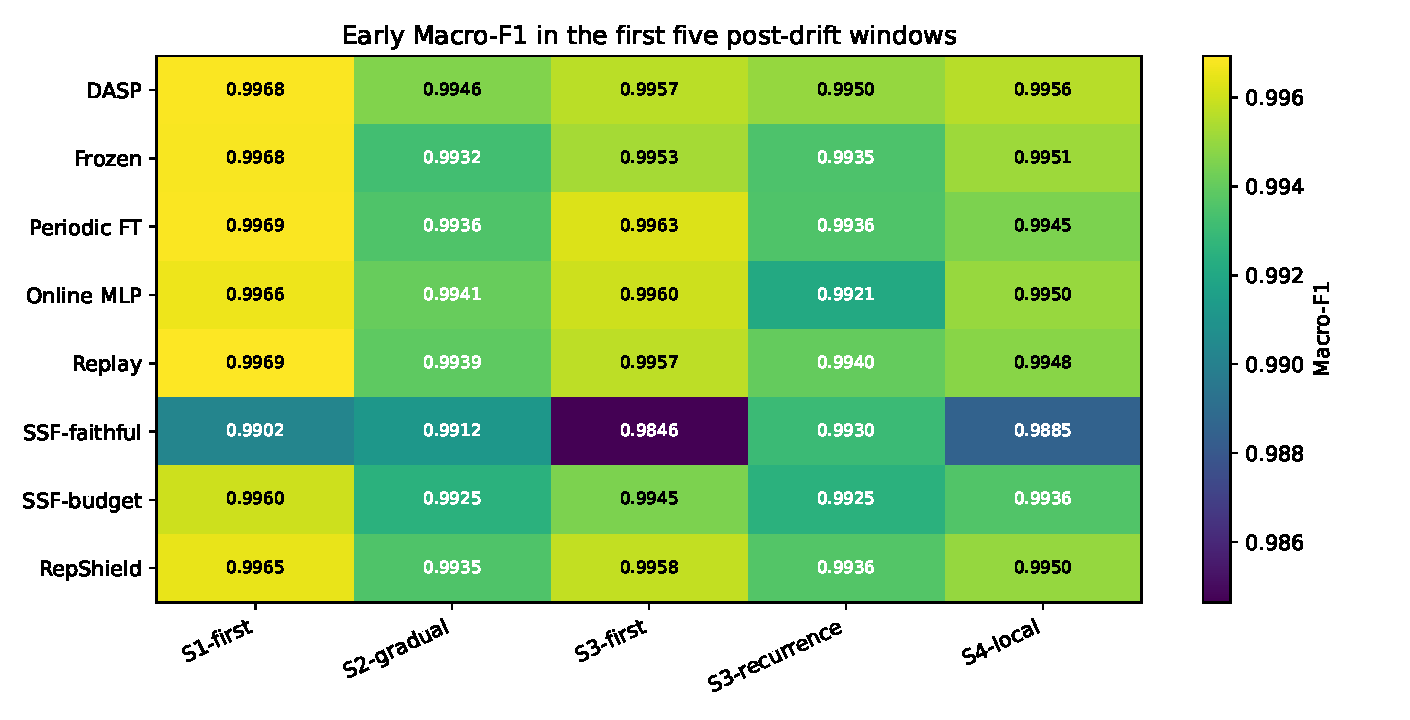
\includegraphics[width=0.92\textwidth]{nf_unsw_drift_episode_heatmap.pdf}
\caption{Mean early macro-F1 over the first five post-shift windows. S3 first shift and recurrence are reported separately. Values are descriptive episode means; paired stream-level intervals and cluster tests determine inferential claims.}
\label{fig:drift_heatmap}
\end{figure*}

\subsection{Shift Type, Recurrence, and Recovery}

Figure \ref{fig:drift_heatmap} shows that all methods operate near the binary-task ceiling. DASP leads S2, S3 recurrence, and S4 among the displayed means, while Experience Replay is slightly higher in S1 and S3 first shift. For DASP, S3 \earlyf{} changes from 0.995651 at first shift to 0.995014 at recurrence, a recurrence gain of $-0.000638$. Attack recall changes from 0.991946 to 0.989140 ($-0.002805$). The decline is small but does not support a recurrence-improvement claim.

The preregistered recovery time is zero for every method because the first post-drift score already exceeds 90\% of the high pre-drift reference. Recovery deficit is likewise zero. These outcomes are ceiling-limited and do not discriminate adaptation on this binary NF-UNSW stream; early F1, early attack recall, and the post-drift minimum are therefore the informative outcomes.

\subsection{Detector Behavior and Stationary Activity}

Detector totals are deduplicated at the run level before aggregation. DASP matched 9 of 50 controlled drift events, producing precision 0.1667, recall 0.1800, and mean matched delay 4.22 windows. Table \ref{tab:detector} also shows that high-recall comparator triggers incur many signals outside the matching region. Trigger definitions differ across methods, so these counts diagnose their executed mechanisms rather than establish a universal detector ranking.

\begin{table}[t]
\caption{Run-Level Drift-Event Matching}
\label{tab:detector}
\centering
\scriptsize
\begin{tabular}{lrrrr}
\toprule
Method & Precision & Recall & False alarms & Delay \\
\midrule
DASP & 0.1667 & 0.1800 & 45 & 4.22 \\
SSF-budget & 0.1318 & 0.5800 & 191 & 0.69 \\
SSF-faithful & 0.0635 & 0.9800 & 723 & 0.31 \\
RepShield & 0.0428 & 1.0000 & 1,117 & 0.02 \\
\bottomrule
\end{tabular}
\end{table}

Across 320 evaluated S0 windows, DASP adapted in 7.1875\% and emitted an alarm or fast trigger in 4.6875\%. It used 24,896 ground-truth update labels across the ten stationary runs, versus 81,920 for the always-updating methods. This supports selectivity and reduced label use, but it does not rescue the weak event-matching recall.

\subsection{GPU Latency, Throughput, and Memory}

Table \ref{tab:systems} separates isolated forward inference from complete test-then-train operation. DASP has the fastest p95 forward inference, 3.675 ms/window, 1.32$\times$ faster than the next method, Periodic FT. This result is consistent with the fused inference cache. DASP nevertheless ranks fifth in mean complete latency because its selective events have a long update tail: 47.558 ms mean and 298.144 ms p95.

\begin{table*}[t]
\caption{Clean GPU Systems Benchmark (Median Run-Level Summaries)}
\label{tab:systems}
\centering
\scriptsize
\setlength{\tabcolsep}{4.0pt}
\begin{tabular}{lrrrrr}
\toprule
Method & p95 forward & Mean complete & p95 complete & Complete throughput & Peak CUDA \\
 & (ms/window) & (ms/window) & (ms/window) & (flows/s) & allocated (MiB) \\
\midrule
Frozen & 6.030 & \textbf{9.597} & 12.819 & \textbf{427,868} & 73.64 \\
Online MLP & 6.201 & 28.536 & 32.412 & 143,690 & 73.64 \\
Periodic FT & 4.855 & 34.012 & 46.009 & 120,492 & 73.64 \\
Experience Replay & 6.236 & 45.206 & 58.881 & 90,613 & 73.64 \\
DASP & \textbf{3.675} & 47.558 & 298.144 & 87,041 & 82.33 \\
SSF-faithful & 6.668 & 414.464 & 474.516 & 9,897 & 75.93 \\
SSF-budget & 6.273 & 428.194 & 490.389 & 9,566 & 75.93 \\
RepShield & 11.205 & 1,205.065 & 1,526.875 & 3,494 & 79.04 \\
\bottomrule
\end{tabular}
\end{table*}

DASP is 5.20\% slower than Experience Replay in mean complete latency, but 8.71$\times$, 9.00$\times$, and 25.34$\times$ faster than SSF-faithful, SSF-budget, and RepShield, respectively. Its median adaptation-event rate is 0.090625 and its median ground-truth update use is 2,624 labels per run, compared with 8,192 for every-window updating methods. The cost is memory: DASP has the largest peak allocated CUDA memory (82.33 MiB) and a 94 MiB peak reserved footprint.

\begin{figure*}[!t]
\centering
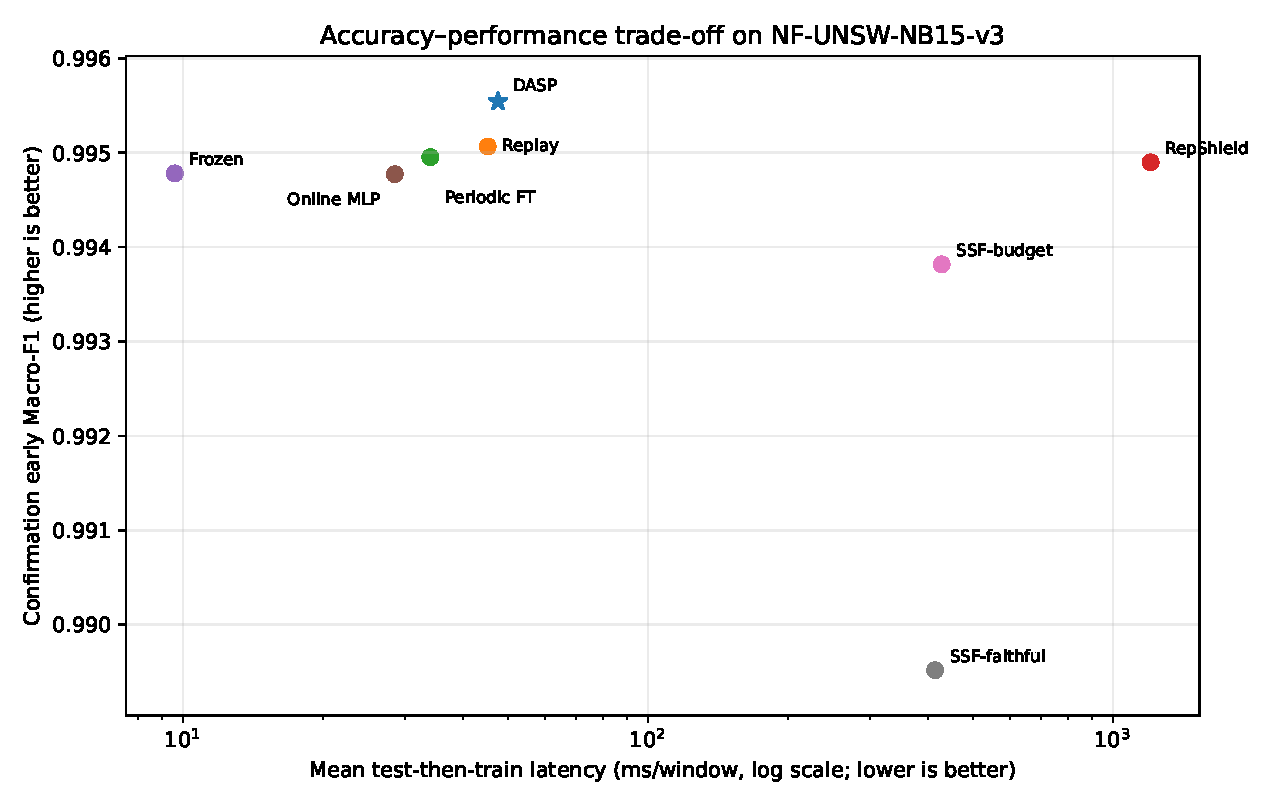
\includegraphics[width=0.88\textwidth]{nf_unsw_accuracy_performance_tradeoff.pdf}
\caption{Confirmation early macro-F1 versus mean complete test-then-train latency from the separate GPU benchmark. The horizontal axis is logarithmic. Higher and farther left is preferable; accuracy and systems evidence come from separate prespecified matrices.}
\label{fig:tradeoff}
\end{figure*}

One CUDA SVD batch used PyTorch's more accurate fallback solver after the default solver did not converge. No run crashed or was retried. The executed fallback time is retained because it is part of the comparator's realized computation.

\section{Discussion}
\label{sec:discussion}

\discussionhead{A. PREDICTIVE ACCURACY WITHOUT UNIVERSAL SUPERIORITY}

DASP attains the highest observed mean early macro-F1 and has positive descriptive bootstrap intervals against six comparators. However, the primary exact stream-cluster test is $p=0.0625$, the Replay interval crosses zero, and no exploratory comparison survives Holm correction. The inferential gate therefore remains closed. The correct conclusion is ``highest observed mean in this matrix with small estimated effects,'' not a supported pairwise or universal superiority claim.

SSF-faithful exposes a second trade-off. It has substantially lower macro-F1 and post-shift minimum, yet the highest attack recall. DASP's estimated recall difference is $-0.004887$, smaller than the planned 0.01 non-inferiority margin in magnitude, but the current completed matrix did not implement the cross-dataset non-inferiority analysis. No recall non-inferiority claim is made.

\discussionhead{B. ACCURACY DOES NOT VALIDATE THE DETECTOR}

DASP detector recall is 0.18 and precision is 0.1667. Its high predictive scores therefore cannot be attributed to reliable one-to-one event detection; they may arise from the strong warm-up model, fast-path behavior, guarded memory refresh, or other components. The completed matrix lacks detector-off and oracle-trigger ablations, so the relative contribution of these mechanisms remains unresolved. The detector is particularly difficult to validate under a near-ceiling binary stream: performance may stay above the recovery floor even when the controlled distribution changes.

Recurrence is similarly nuanced. DASP has the highest mean S3 recurrence F1 among the locked methods, but its own recurrence gain is slightly negative. This supports retention relative to several comparators, not improvement over its first-drift state. Better detector evidence requires streams that produce a material binary decision-boundary change and include localized minority degradation.

\discussionhead{C. FUSED FORWARD SPEED VERSUS UPDATE TAIL}

The fused inference cache succeeds at its intended purpose. DASP is first of eight methods in p95 forward inference. Complete service cost tells a different story: event updates create a 298-ms p95 tail, placing DASP fifth in mean test-then-train latency. This distinction is operationally important. A deployment that performs inference and adaptation on separate workers may benefit from the 3.675-ms forward path, whereas a single synchronous worker must provision for update stalls.

DASP is far faster end-to-end than both SSF forms and RepShield, uses fewer labels, and adapts in fewer windows. It is not faster than Frozen, Online MLP, Periodic FT, or Replay in complete operation, and it has the largest allocated GPU footprint. The evidence therefore supports selective computational efficiency relative to expensive continual methods, not global systems dominance.

\discussionhead{D. EVIDENCE SCOPE}

This confirmation covers one dataset and binary classification. It is statistically paired across five stream seeds and two model seeds, but only the stream seeds are independent replication units. The exact test consequently has coarse resolution and the primary $p=0.0625$ does not establish superiority. The cross-dataset protocol remains the appropriate next evaluation: NF-CSE-CIC-IDS2018-v3, NF-ToN-IoT-v3, NF-BoT-IoT-v3, and LUFlow must be executed with the same current DASP code before any broad claim is restored. Multiclass attack-family drift is also untested.

\section{Threats to Validity and Limitations}
\label{sec:limitations}

\textbf{Construct validity:} The controlled generator creates known changes in attack-family composition while holding attack prevalence fixed, but it does not intervene directly on $P(Y\mid X)$. On the confirmation streams, the A-trained probe did not degrade on B, and NF-UNSW binary performance is near ceiling. These episodes are therefore evidence of class-conditional distribution shift, not verified real concept drift. Zero recovery times further show that the perturbations do not create a sufficiently harmful binary decision shift.

\textbf{Internal validity:} All methods share paired streams, initializations, delay, and ground-truth budgets. Published baselines still require implementation choices. SSF-faithful and SSF-budget are separated to disclose pseudo-label differences. Trigger counts are mechanism-specific and should not be interpreted as measurements from an identical detector. Because detector-off and oracle-trigger ablations were not run in this matrix, the predictive effect of the proposed trigger is not causally identified.

\textbf{Statistical conclusion validity:} Five stream seeds and two nested model seeds provide paired confirmation within NF-UNSW, but there is only one dataset. Hierarchical-bootstrap intervals quantify conditional stream-seed uncertainty, not dataset-level generalization. The exact sign-flip test over five stream clusters did not reach 0.05, and no exploratory contrast survived Holm correction. Near-ceiling values compress effect sizes. Windows and nested model seeds are not independent samples.

\textbf{External validity:} Results may change with other IDS datasets, longer label delays, partial labels, new attack classes, encrypted traffic, different backbones, natural chronological streams, or multiclass tasks. The previous five-dataset and chronological outputs belong to earlier DASP implementations and are not pooled with the current confirmation.

\textbf{Systems validity:} Timing comes from one Windows laptop GPU with two PyTorch CPU threads. Energy, concurrent packet capture, transfer overlap, queueing, and multi-tenant interference were not measured. The 80-run systems matrix uses one stream seed and two model seeds; it characterizes the tested implementation rather than a hardware-independent complexity bound. The SVD fallback is disclosed because it affects realized comparator time.

\section{Conclusion}
\label{sec:conclusion}

DASP performs prediction-first selective adaptation through low-rank layer branches, feature-wise modulation, current-batch similarity replay, class-balanced guards, and a fused inference cache while leaving the base hidden blocks frozen after warm-up. In 400 locked NF-UNSW-NB15-v3 runs, DASP achieved the highest mean early macro-F1, but the primary exact stream-cluster test gave $p=0.0625$ and no exploratory comparison survived Holm correction. The controlled artifacts changed attack-family distributions without degrading an A-trained binary probe, so they do not verify real concept drift. DASP's detector precision and recall remain weak, its causal trigger benefit is untested, and recurrence is slightly below its own first-shift performance.

The 80-run GPU benchmark establishes a systems trade-off. DASP has the fastest p95 forward inference but ranks fifth in complete test-then-train latency, is slightly slower than Replay, and uses the most allocated CUDA memory. It is nevertheless substantially faster than SSF and RepShield while using fewer labels and adapting in fewer windows. The defensible conclusion is that DASP is an accurate, selective, and fast-forward streaming design under this single-dataset distribution-shift evaluation, with unresolved trigger quality and update-tail costs. Boundary-impacting, cross-dataset, causal-ablation, and natural-stream confirmation are required before a broader state-of-the-art claim.

\section*{Data Availability}

The source NF-UNSW-NB15-v3 data are publicly available from the NF-v3 dataset providers \cite{Luay2025NetFlowV3,UQNIDSDatasets2025}. The 400-run confirmation is stored under \path{outputs_dasp_fast_nf_unsw_locked_7_gpu}; the CUDA-synchronized 80-run systems benchmark is stored under \path{outputs_dasp_fast_nf_unsw_locked7_performance_gpu_v2}; and the integrated drift/performance tables and figures are stored under \path{outputs_dasp_fast_nf_unsw_locked_7_gpu/analysis_locked7_drift_performance}. A public archival repository and persistent identifier must be added before submission.

\section*{Ethics Statement}

This study analyzes public, de-identified network-flow benchmark data and performs no intervention on a live network. It involves no human participants, private records, or personal-contact data. Dataset use and redistribution must follow the source licenses.

\section*{Author Contributions}

The authors must replace this placeholder with a verified CRediT statement. Relevant roles include conceptualization, methodology, software, validation, formal analysis, data curation, visualization, writing--original draft, writing--review and editing, supervision, and project administration.

\section*{Funding}

Funding information must be completed and verified by the authors. No funding source is asserted in this draft.

\section*{Conflict of Interest}

Conflict-of-interest information must be verified by every author. No competing-interest declaration is inferred by the manuscript preparation workflow.

\section*{Declaration of Generative AI and AI-Assisted Technologies}

Generative AI tools assisted manuscript organization, language editing, code inspection, and reproducibility checks. The study design, algorithm choices, execution, interpretation, and final claims remain the responsibility of the authors. The authors must verify every numerical result, citation, and statement before submission.

\appendices

\section{Locked Configuration and Reproducibility Record}
\label{app:config}

\textbf{Model and stream:} The binary runner uses 49 numeric inputs, hidden widths 256--128--64, 36 windows of 4,096 flows, four warm-up windows, batch size 256, AdamW learning rate $10^{-3}$, weight decay $10^{-4}$, one-window label delay, memory capacity 5,000, and a maximum of 256 ground-truth update labels per window.

\textbf{DASP configuration:} The adapter maximum rank is 32; fast and strong ranks are 4 and 32. The fast path uses one epoch and 128 replay samples; the strong path uses two epochs, 256 replay samples, and a five-window recovery horizon. Feature modulation scale is 0.5. The input adapter dimension is 16. Similarity replay uses a 512-flow query, temperature 0.10, confidence power 1, and an adaptive uniform mixture bounded by 0.75. Candidate commit fractions are 1 and 0.5. The guard history is 512; tolerances are 0 for macro-F1 and $-0.01$ for attack and minimum-class recall.

\textbf{Detector:} Multilevel MMD uses 192 samples, scales $\{0.5,1,2\}$, threshold 0.15, emergency threshold 0.60, and persistence 2. The fast input gate threshold is 0.075. The performance trigger uses five reference windows, a four-observation minimum history, 0.08 macro-F1 and recall drops, and a cooldown of two.

\textbf{Matrices and audits:} The confirmation manifest records one dataset, five scenarios, five stream seeds, two model seeds, eight methods, and 400/400 completed runs. The systems manifest records five scenarios, one stream seed, two model seeds, eight methods, and 80/80 completed runs. The clean systems audit reports zero duplicate keys, exact method and scenario counts, finite primary timings, and zero DASP global-update violations. The software suite passed 102/102 tests in the locked NumPy 1.26.4/PyTorch 2.3.1 environment after the construct, S5-control, and cluster-inference checks were added.

\bibliographystyle{IEEEtran}
\bibliography{references}

\EOD
\end{document}
